\documentclass[10pt]{amsart}
\usepackage{amsmath}
\usepackage{amssymb}
\usepackage{tikz}
\usetikzlibrary{decorations.markings}
\usepackage{xcolor}
\usepackage{color}
\usepackage[color,all]{xy}

\newcommand{\cF}{\mathcal{F}}

\begin{document}

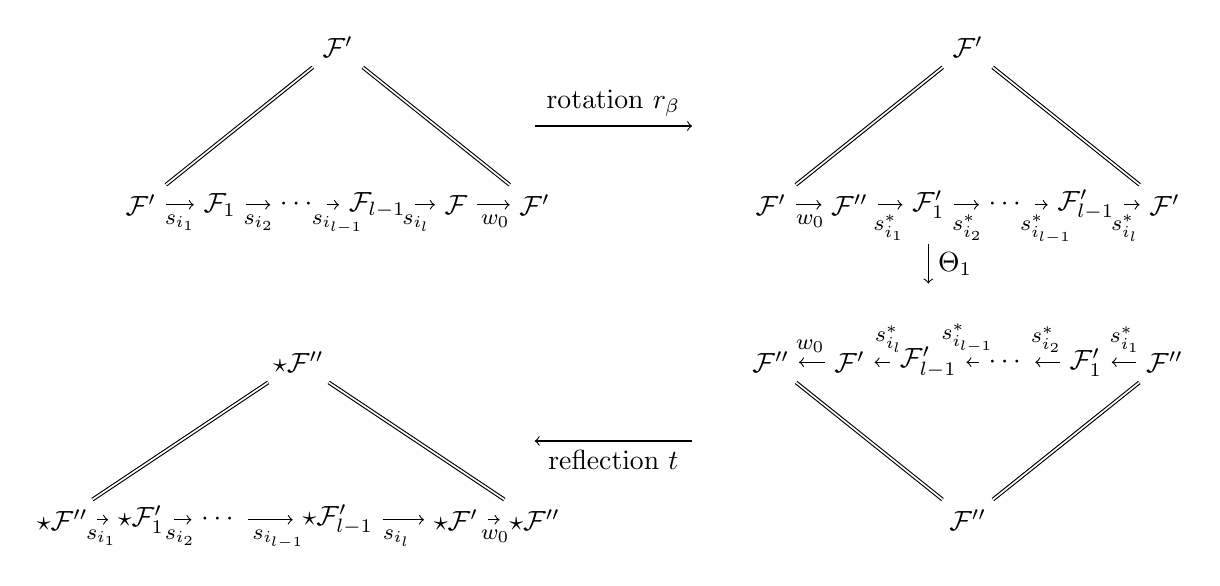
\begin{tikzpicture}[node1/.pic={
\node (0)  at (0,0) [] {$\cF'$};
\node (1) at (1,0) [] {$\cF_1$};
    \node (3) at (3,0) [] {$\cF_{l-1}$};
    \node (2) at (2,0) [] {$\cdots$};
    \node (4) at (4,0) [] {$\cF$};
    \node (a) at (2.5,2) [] {$\cF'$};
    \draw [->] (0) -- (1);
    \draw [->] (1) -- (2);
    \draw [->] (2) -- (3);
    \draw [->] (3) -- (4);
    \node at (0.5,0) [below] {\footnotesize{$s_{i_1}$}};
    \node at (1.5,0) [below] {\footnotesize{$s_{i_2}$}};
    \node at (2.5,0) [below] {\footnotesize{$s_{i_{l-1}}$}};
    \node at (3.5,0) [below] {\footnotesize{$s_{i_l}$}};
    \node (5) at (5,0) [] {$\cF'$};
    \draw [double] (0) -- (a);
    \draw [->] (4) -- (5);
    \draw [double] (a) -- (5);
    \node at (4.5,0) [below] {\footnotesize{$w_0$}};
}, node2/.pic={
    \node (0) at (0,0) [] {$\cF'$};
    \node (1) at (1,0) [] {$\cF''$};
    \node (2) at (2,0) [] {$\cF'_1$};
    \node (3) at (3,0) [] {$\cdots$};
    \node (4) at (4,0) [] {$\cF'_{l-1}$};
    \node (5) at (5,0) [] {$\cF'$};
    \node (a) at (2.5,2) [] {$\cF'$};
    \draw [->] (0) -- (1);
    \draw [->] (1) -- (2);
    \draw [->] (2) -- (3);
    \draw [->] (3) -- (4);
    \draw [->] (4) -- (5);
    \node at (0.5,0) [below] {\footnotesize{$w_0$}};
    \node at (1.5,0) [below] {\footnotesize{$s^*_{i_1}$}};
    \node at (2.5,0) [below] {\footnotesize{$s^*_{i_2}$}};
    \node at (3.5,0) [below] {\footnotesize{$s^*_{i_{l-1}}$}};
    \node at (4.5,0) [below] {\footnotesize{$s^*_{i_l}$}};
    \draw [double] (0) -- (a);
    \draw [double] (5) -- (a);
}, node3/.pic={
    \node (1) at (5,2) [] {$\cF''$};
    \node (2) at (4,2) [] {$\cF'_1$};
    \node (3) at (3,2) [] {$\cdots$};
    \node (4) at (2,2) [] {$\cF'_{l-1}$};
    \node (0) at (1,2) [] {$\cF'$};
    \node (-1) at (0,2) [] {$\cF''$};
    \node (a) at (2.5,0) [] {$\cF''$};
    \draw [->] (4) -- (0);
    \draw [->] (1) -- (2);
    \draw [->] (2) -- (3);
    \draw [->] (3) -- (4);
    \draw [->] (0) -- (-1);
    \node at (4.5,2) [above] {\footnotesize{$s_{i_1}^*$}};
    \node at (3.5,2) [above] {\footnotesize{$s_{i_2}^*$}};
    \node at (2.5,2) [above] {\footnotesize{$s_{i_{l-1}}^*$}};
    \node at (1.5,2) [above] {\footnotesize{$s_{i_l}^*$}};
    \node at (0.5,2) [above] {\footnotesize{$w_0$}};
    \draw [double] (-1) -- (a);
    \draw [double] (a) -- (1);
}, node4/.pic={
    \node (0)  at (0,0) [] {$\star\cF''$};
\node (1) at (1,0) [] {$\star\cF'_1$};
    \node (3) at (3.5,0) [] {$\star\cF'_{l-1}$};
    \node (2) at (2,0) [] {$\cdots$};
    \node (4) at (5,0) [] {$\star\cF'$};
    \node (a) at (3,2) [] {$\star\cF''$};
    \draw [->] (0) -- (1);
    \draw [->] (1) -- (2);
    \draw [->] (2) -- (3);
    \draw [->] (3) -- (4);
    \node at (0.5,0) [below] {\footnotesize{$s_{i_1}$}};
    \node at (1.5,0) [below] {\footnotesize{$s_{i_2}$}};
    \node at (2.75,0) [below] {\footnotesize{$s_{i_{l-1}}$}};
    \node at (4.25,0) [below] {\footnotesize{$s_{i_l}$}};
    \node (5) at (6,0) [] {$\star\cF''$};
    \draw [double] (0) -- (a);
    \draw [->] (4) -- (5);
    \draw [double] (a) -- (5);
    \node at (5.5,0) [below] {\footnotesize{$w_0$}};
}
]
\draw (0,4) pic {node1};
\draw (8,4) pic {node2};
\draw (8,0) pic {node3};
\draw (-1,0) pic {node4};
\draw [->] (7,1) -- node [below] {reflection $t$} (5,1);
\draw [->] (5,5) -- node [above] {rotation $r_\beta$} (7,5);
\draw[->] (10,3.5) -- node [right] {$\Theta_1$} (10,3);
\end{tikzpicture}

\end{document}